\section{Graph Based Problem Formulation}
A solution to the bus charge problem must reveal \textit{what} to charge and \textit{when} to charge it. This implies a two dimensional solution where each axis describes \textit{what} and \textit{when} to charge respectively. The first dimension contains one charge state for each bus and an additional `no-charge' state. The time axis is continuous by nature and is represented discretly by the time indices $t_0,t_1,\hdots,t_n$ 
\par The intersection of each charge state and time index is represented by a node (see figure \ref{fig:graphGridStructure}) where the the $ij^{\text{th}}$ node represents the $i^{\text{th}}$ charge state at the $j^{\text{th}}$ time index. For example, $\text{node}_{1,1}$ of figure \ref{fig:graphGridStructure} represents a state where a charger charges Bus 2 at time index $t_0$. 
\par Note that a complete grid, implies that each charger can charge any bus at any time.  When buses leave the station for routes however, they become unavailable. To reflect the various absenses caused by running routes, charge nodes corresponding to route times must be removed (see figure \ref{fig:busAvailEncode}). 

\begin{figure*}
	\subfloat[Graph showing buses and timesteps \label{fig:graphGridStructure}]{
		\centering
		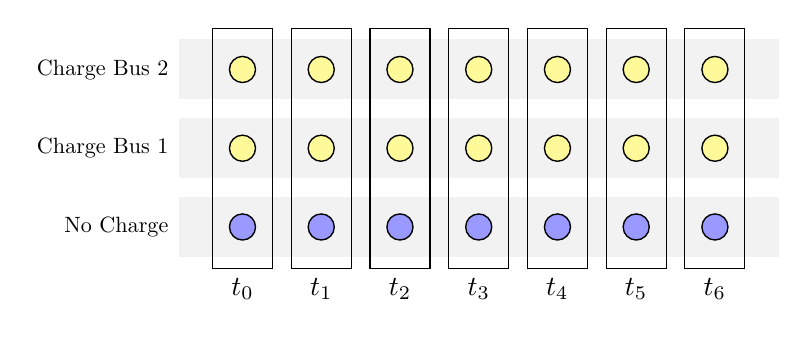
\begin{tikzpicture}
			\node[rectangle, fill=gray!10, minimum width=3in, minimum height=.3in,label=left:\scalebox{0.8}{Charge Bus 2}](bus2Box) at (3,1){};
			\node[rectangle, fill=gray!10, minimum width=3in, minimum height=.3in,label=left:\scalebox{0.8}{Charge Bus 1}](bus1Box) at (3,0){};
			\node[rectangle, fill=gray!10, minimum width=3in, minimum height=.3in,label=left:\scalebox{0.8}{No Charge}](bus1Box) at (3,-1){};

			\node[circle, fill=yellow!40, line width=0.5pt, draw=black, minimum size=0.1in](one) at (0,0){};
			\node[circle, fill=yellow!40, line width=0.5pt, draw=black, minimum size=0.1in](two) at (1,0){}; 
			\node[circle, fill=yellow!40, line width=0.5pt, draw=black, minimum size=0.1in](three) at (2,0){};
			\node[circle, fill=yellow!40, line width=0.5pt, draw=black, minimum size=0.1in](four) at (3,0){};
			\node[circle, fill=yellow!40, line width=0.5pt, draw=black, minimum size=0.1in](five) at (4,0){};
			\node[circle, fill=yellow!40, line width=0.5pt, draw=black, minimum size=0.1in](six) at (5,0){};
			\node[circle, fill=yellow!40,  line width=0.5pt, draw=black, minimum size=0.1in](seven) at (6,0){};

			\node[circle, fill=yellow!40, line width=0.5pt, draw=black, minimum size=0.1in](eight) at (0,1){};
			\node[circle, fill=yellow!40, line width=0.5pt, draw=black, minimum size=0.1in](nine) at (1,1){}; 
			\node[circle, fill=yellow!40, line width=0.5pt, draw=black, minimum size=0.1in](ten) at (2,1){};
			\node[circle, fill=yellow!40, line width=0.5pt, draw=black, minimum size=0.1in](eleven) at (3,1){};
			\node[circle, fill=yellow!40, line width=0.5pt, draw=black, minimum size=0.1in](twelve) at (4,1){};
			\node[circle, fill=yellow!40, line width=0.5pt, draw=black, minimum size=0.1in](thirteen) at (5,1){};
			\node[circle, fill=yellow!40, line width=0.5pt, draw=black, minimum size=0.1in](fourteen) at (6,1){};

			\node[circle, fill=blue!40, line width=0.5pt, draw=black, minimum size=0.1in](eight) at (0,-1){};
			\node[circle, fill=blue!40, line width=0.5pt, draw=black, minimum size=0.1in](nine) at (1,-1){}; 
			\node[circle, fill=blue!40, line width=0.5pt, draw=black, minimum size=0.1in](ten) at (2,-1){};
			\node[circle, fill=blue!40, line width=0.5pt, draw=black, minimum size=0.1in](eleven) at (3,-1){};
			\node[circle, fill=blue!40, line width=0.5pt, draw=black, minimum size=0.1in](twelve) at (4,-1){};
			\node[circle, fill=blue!40, line width=0.5pt, draw=black, minimum size=0.1in](thirteen) at (5,-1){};
			\node[circle, fill=blue!40, line width=0.5pt, draw=black, minimum size=0.1in](fourteen) at (6,-1){};

			\node[rectangle, draw, minimum width=0.3in, minimum height=1.2in,label=below:$t_0$](time0Box) at (0,0){};
			\node[rectangle, draw, minimum width=0.3in, minimum height=1.2in,label=below:$t_1$](time1Box) at (1,0){};
			\node[rectangle, draw, minimum width=0.3in, minimum height=1.2in,label=below:$t_2$](time2Box) at (2,0){};
			\node[rectangle, draw, minimum width=0.3in, minimum height=1.2in,label=below:$t_3$](time3Box) at (3,0){};
			\node[rectangle, draw, minimum width=0.3in, minimum height=1.2in,label=below:$t_4$](time4Box) at (4,0){};
			\node[rectangle, draw, minimum width=0.3in, minimum height=1.2in,label=below:$t_5$](time5Box) at (5,0){};
			\node[rectangle, draw, minimum width=0.3in, minimum height=1.2in,label=below:$t_6$](time6Box) at (6,0){}; 
		\end{tikzpicture}
	}
	\subfloat[two-bus scenario from figure \ref{fig:graphGridStructure} where each bus is absent at $t_0$, $t_3$, and $t_6$ \label{fig:busAvailEncode}]{
		\centering
		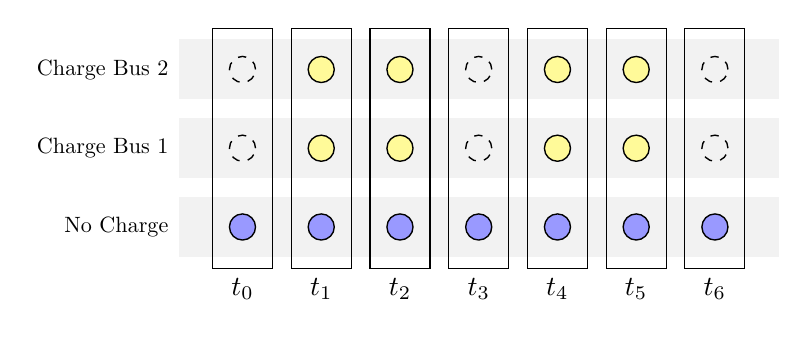
\begin{tikzpicture} 
			\node[rectangle, fill=gray!10, minimum width=3in, minimum height=.3in,label=left:\scalebox{0.8}{Charge Bus 2}](bus2Box) at (3,1){};
			\node[rectangle, fill=gray!10, minimum width=3in, minimum height=.3in,label=left:\scalebox{0.8}{Charge Bus 1}](bus1Box) at (3,0){};
			\node[rectangle, fill=gray!10, minimum width=3in, minimum height=.3in,label=left:\scalebox{0.8}{No Charge}](bus1Box) at (3,-1){};

			\node[circle, draw, dashed, line width=0.5pt, draw=black, minimum size=0.1in](one) at (0,0){};
			\node[circle, fill=yellow!40, line width=0.5pt, draw=black, minimum size=0.1in](two) at (1,0){}; 
			\node[circle, fill=yellow!40, line width=0.5pt, draw=black, minimum size=0.1in](three) at (2,0){};
			\node[circle, draw, dashed, line width=0.5pt, draw=black, minimum size=0.1in](four) at (3,0){};
			\node[circle, fill=yellow!40, line width=0.5pt, draw=black, minimum size=0.1in](five) at (4,0){};
			\node[circle, fill=yellow!40, line width=0.5pt, draw=black, minimum size=0.1in](six) at (5,0){};
			\node[circle, draw, dashed,  line width=0.5pt, draw=black, minimum size=0.1in](seven) at (6,0){};

			\node[circle, draw, dashed, line width=0.5pt, draw=black, minimum size=0.1in](eight) at (0,1){};
			\node[circle, fill=yellow!40, line width=0.5pt, draw=black, minimum size=0.1in](nine) at (1,1){}; 
			\node[circle, fill=yellow!40, line width=0.5pt, draw=black, minimum size=0.1in](ten) at (2,1){};
			\node[circle, draw, dashed, line width=0.5pt, draw=black, minimum size=0.1in](eleven) at (3,1){};
			\node[circle, fill=yellow!40, line width=0.5pt, draw=black, minimum size=0.1in](twelve) at (4,1){};
			\node[circle, fill=yellow!40, line width=0.5pt, draw=black, minimum size=0.1in](thirteen) at (5,1){};
			\node[circle, draw, dashed, line width=0.5pt, draw=black, minimum size=0.1in](fourteen) at (6,1){};

			\node[circle, fill=blue!40, line width=0.5pt, draw=black, minimum size=0.1in](eight) at (0,-1){};
			\node[circle, fill=blue!40, line width=0.5pt, draw=black, minimum size=0.1in](nine) at (1,-1){}; 
			\node[circle, fill=blue!40, line width=0.5pt, draw=black, minimum size=0.1in](ten) at (2,-1){};
			\node[circle, fill=blue!40, line width=0.5pt, draw=black, minimum size=0.1in](eleven) at (3,-1){};
			\node[circle, fill=blue!40, line width=0.5pt, draw=black, minimum size=0.1in](twelve) at (4,-1){};
			\node[circle, fill=blue!40, line width=0.5pt, draw=black, minimum size=0.1in](thirteen) at (5,-1){};
			\node[circle, fill=blue!40, line width=0.5pt, draw=black, minimum size=0.1in](fourteen) at (6,-1){};

			\node[rectangle, draw, minimum width=0.3in, minimum height=1.2in,label=below:$t_0$](time0Box) at (0,0){};
			\node[rectangle, draw, minimum width=0.3in, minimum height=1.2in,label=below:$t_1$](time1Box) at (1,0){};
			\node[rectangle, draw, minimum width=0.3in, minimum height=1.2in,label=below:$t_2$](time2Box) at (2,0){};
			\node[rectangle, draw, minimum width=0.3in, minimum height=1.2in,label=below:$t_3$](time3Box) at (3,0){};
			\node[rectangle, draw, minimum width=0.3in, minimum height=1.2in,label=below:$t_4$](time4Box) at (4,0){};
			\node[rectangle, draw, minimum width=0.3in, minimum height=1.2in,label=below:$t_5$](time5Box) at (5,0){};
			\node[rectangle, draw, minimum width=0.3in, minimum height=1.2in,label=below:$t_6$](time6Box) at (6,0){}; 
		\end{tikzpicture}
	}
		\caption{Bus availability represented in a graph}
\end{figure*}

\par Additionally, charge nodes are only valid for small periods of time. As time progresses, chargers must transition from state to state. These state transitions are represented by forming a weighted connection, or edge between two nodes (see figure \ref{fig:edgeNodeRel}). Each edge leaves a previous state and enters a target state. The use of each edge is determined by its weight, which gives the number of chargers using the transition.  Therefore edges by themselves represent \textit{potential} transitions (see figure \ref{fig:completeGraph}), and are made `active' by assigning a non-zero weight.  
\begin{figure}
	\centering
	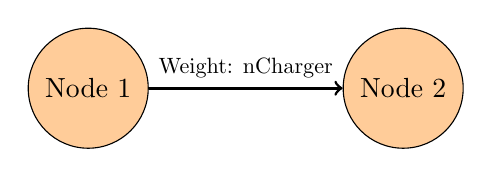
\begin{tikzpicture}
		\node[circle, draw, fill=orange!40, minimum size=0.6in](node1) at (0,0){Node 1};
		\node[circle, draw, fill=orange!40, minimum size=0.6in](node2) at (4,0){Node 2};
		\draw [->, line width=1pt] (node1.east) -- node[above]{\scalebox{0.8}{Weight: nCharger}}(node2.west); 
	\end{tikzpicture}
	\caption{Node to Node Connection}
	\label{fig:edgeNodeRel}
\end{figure}

\begin{figure}
	\centering
	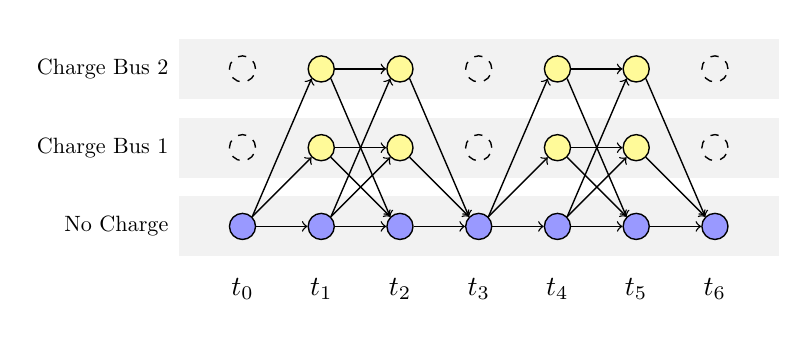
\begin{tikzpicture} 
		\node[rectangle, fill=gray!10, minimum width=3in, minimum height=.3in,label=left:\scalebox{0.8}{Charge Bus 2}](bus2Box) at (3,1){};
		\node[rectangle, fill=gray!10, minimum width=3in, minimum height=.3in,label=left:\scalebox{0.8}{Charge Bus 1}](bus1Box) at (3,0){};
		\node[rectangle, fill=gray!10, minimum width=3in, minimum height=.3in,label=left:\scalebox{0.8}{No Charge}](bus1Box) at (3,-1){};

		\node[circle, draw, dashed, line width=0.5pt, draw=black, minimum size=0.1in](one) at (0,0){};
		\node[circle, fill=yellow!40, line width=0.5pt, draw=black, minimum size=0.1in](two) at (1,0){}; 
		\node[circle, fill=yellow!40, line width=0.5pt, draw=black, minimum size=0.1in](three) at (2,0){};
		\node[circle, draw, dashed, line width=0.5pt, draw=black, minimum size=0.1in](four) at (3,0){};
		\node[circle, fill=yellow!40, line width=0.5pt, draw=black, minimum size=0.1in](five) at (4,0){};
		\node[circle, fill=yellow!40, line width=0.5pt, draw=black, minimum size=0.1in](six) at (5,0){};
		\node[circle, draw, dashed,  line width=0.5pt, draw=black, minimum size=0.1in](seven) at (6,0){};

		\node[circle, draw, dashed, line width=0.5pt, draw=black, minimum size=0.1in](eight) at (0,1){};
		\node[circle, fill=yellow!40, line width=0.5pt, draw=black, minimum size=0.1in](nine) at (1,1){}; 
		\node[circle, fill=yellow!40, line width=0.5pt, draw=black, minimum size=0.1in](ten) at (2,1){};
		\node[circle, draw, dashed, line width=0.5pt, draw=black, minimum size=0.1in](eleven) at (3,1){};
		\node[circle, fill=yellow!40, line width=0.5pt, draw=black, minimum size=0.1in](twelve) at (4,1){};
		\node[circle, fill=yellow!40, line width=0.5pt, draw=black, minimum size=0.1in](thirteen) at (5,1){};
		\node[circle, draw, dashed, line width=0.5pt, draw=black, minimum size=0.1in](fourteen) at (6,1){};

		\node[circle, fill=blue!40, line width=0.5pt, draw=black, minimum size=0.1in](bOne) at (0,-1){};
		\node[circle, fill=blue!40, line width=0.5pt, draw=black, minimum size=0.1in](bTwo) at (1,-1){}; 
		\node[circle, fill=blue!40, line width=0.5pt, draw=black, minimum size=0.1in](bThree) at (2,-1){};
		\node[circle, fill=blue!40, line width=0.5pt, draw=black, minimum size=0.1in](bFour) at (3,-1){};
		\node[circle, fill=blue!40, line width=0.5pt, draw=black, minimum size=0.1in](bFive) at (4,-1){};
		\node[circle, fill=blue!40, line width=0.5pt, draw=black, minimum size=0.1in](bSix) at (5,-1){};
		\node[circle, fill=blue!40, line width=0.5pt, draw=black, minimum size=0.1in](bSeven) at (6,-1){};

		\node[rectangle, minimum width=0.3in, minimum height=1.2in,label=below:$t_0$](time0Box) at (0,0){};
		\node[rectangle, minimum width=0.3in, minimum height=1.2in,label=below:$t_1$](time1Box) at (1,0){};
		\node[rectangle, minimum width=0.3in, minimum height=1.2in,label=below:$t_2$](time2Box) at (2,0){};
		\node[rectangle, minimum width=0.3in, minimum height=1.2in,label=below:$t_3$](time3Box) at (3,0){};
		\node[rectangle, minimum width=0.3in, minimum height=1.2in,label=below:$t_4$](time4Box) at (4,0){};
		\node[rectangle, minimum width=0.3in, minimum height=1.2in,label=below:$t_5$](time5Box) at (5,0){};
		\node[rectangle, minimum width=0.3in, minimum height=1.2in,label=below:$t_6$](time6Box) at (6,0){}; 
		
		% draw rest edges
		\draw[->, line width=0.5pt] (bOne.east) -- (bTwo.west);
		\draw[->, line width=0.5pt] (bTwo.east) -- (bThree.west);
		\draw[->, line width=0.5pt] (bThree.east) -- (bFour.west);
		\draw[->, line width=0.5pt] (bFour.east) -- (bFive.west);
		\draw[->, line width=0.5pt] (bFive.east) -- (bSix.west);
		\draw[->, line width=0.5pt] (bSix.east) -- (bSeven.west);
		
		% draw connect edges
		\draw[->, line width=0.5pt] (bOne.north east) -- (two.south west); 
		\draw[->, line width=0.5pt] (bTwo.north east) -- (three.south west);
		\draw[->, line width=0.5pt] (bFour.north east) -- (five.south west);
		\draw[->, line width=0.5pt] (bFive.north east) -- (six.south west);

		\draw[->, line width=0.5pt] (bOne.north east) -- (nine.south west);
		\draw[->, line width=0.5pt] (bTwo.north east) -- (ten.south west);
		\draw[->, line width=0.5pt] (bFour.north east) -- (twelve.south west);
		\draw[->, line width=0.5pt] (bFive.north east) -- (thirteen.south west);

		% draw disconnect edges
		\draw[->, line width=0.5pt] (two.south east) -- (bThree.north west); 
		\draw[->, line width=0.5pt] (three.south east) -- (bFour.north west);
		\draw[->, line width=0.5pt] (five.south east) -- (bSix.north west);
		\draw[->, line width=0.5pt] (six.south east) -- (bSeven.north west);

		\draw[->, line width=0.5pt] (nine.south east) -- (bThree.north west);
		\draw[->, line width=0.5pt] (ten.south east) -- (bFour.north west);
		\draw[->, line width=0.5pt] (twelve.south east) -- (bSix.north west);
		\draw[->, line width=0.5pt] (thirteen.south east) -- (bSeven.north west);

		% draw charge edges
		\draw[->, line width=0.5pt] (two.east) -- (three.west);
		\draw[->, line width=0.5pt] (five.east) -- (six.west);
		\draw[->, line width=0.5pt] (nine.east) -- (ten.west);
		\draw[->, line width=0.5pt] (twelve.east) -- (thirteen.west);

	\end{tikzpicture}
	\caption{Complete Problem formulation}
	\label{fig:completeGraph}
\end{figure}
\par Edges can also be thought of as decisions because they determine the next state for each charger. In the bus charge problem, there are four types of decisions: Connect, Charge, No-Charge, and Disconnect. Connect edges are formed when an edge transitions from a no-charge state to a charge state, charge edges are given by connections from one charge state to another, No-Charge transitions occur between no-charge nodes, and disconnect edges transition from charge to no-charge states (see figure \ref{fig:edgeTypes}).
\begin{figure}
	\centering
	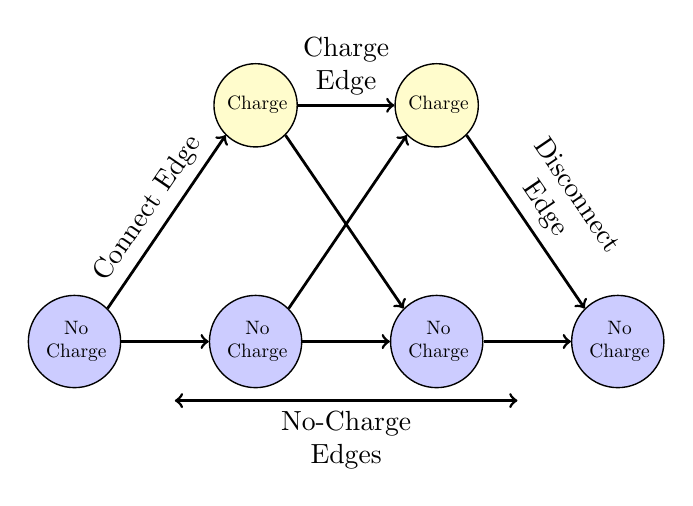
\begin{tikzpicture}
		\node[circle, fill=blue!20,line width=0.5pt, draw=black, text width=0.4in, inner sep=0in](one) at (0,0){\scalebox{0.7}{\begin{tabular}{c}No\\ Charge \end{tabular}}};
		\node[circle, fill=blue!20,line width=0.5pt, draw=black, text width=0.4in, inner sep=0in](two) at (2.3,0){\scalebox{0.7}{\begin{tabular}{c}No\\ Charge \end{tabular}}};
		\node[circle, fill=blue!20,line width=0.5pt, draw=black, text width=0.4in, inner sep=0in](three) at (4.6,0){\scalebox{0.7}{\begin{tabular}{c}No\\ Charge \end{tabular}}};
		\node[circle, fill=blue!20,line width=0.5pt, draw=black, text width=0.4in, inner sep=0in](four) at (6.9,0){\scalebox{0.7}{\begin{tabular}{c}No\\ Charge \end{tabular}}};
		\node[circle, fill=yellow!20,line width=0.5pt, draw=black, text width=0.4in, inner sep=0in](five) at (2.3,3){\scalebox{0.7}{\begin{tabular}{c} Charge \end{tabular}}};
		\node[circle, fill=yellow!20,line width=0.5pt, draw=black, text width=0.4in, inner sep=0in](six) at (4.6,3){\scalebox{0.7}{\begin{tabular}{c}Charge \end{tabular}}};
		\node(placeholder1) at (1.15,-0.75){};
		\node(placeholder2) at (5.75,-0.75){};
		\draw [->, line width=1pt] (one.north east) -- node[sloped, anchor=center, above, text width=2.5cm, midway, align=center]{Connect Edge}(five.south west);
		\draw [->, line width=1pt] (one.east) -- (two.west);
		\draw [->, line width=1pt] (five.east) -- node[sloped, anchor=center, above, text width=1.5cm, midway, align=center]{Charge Edge}(six.west);
		\draw [->, line width=1pt] (five.south east) -- (three.north west);
		\draw [->, line width=1pt] (two.north east) -- (six.south west);
		\draw [->, line width=1pt] (six.south east) -- node[sloped, anchor=center, above, text width=1.5cm, midway, align=center]{Disconnect Edge}(four.north west);
		\draw [->, line width=1pt] (two.east) -- (three.west);
		\draw [->, line width=1pt] (three.east) -- (four.west); 
		\draw [<->, line width=1pt] (placeholder1) -- node[below, text width=2cm, midway, align=center]{No-Charge Edges}(placeholder2);
	\end{tikzpicture}
	\caption{Connect, Disconnect, and Charge Edges}
	\label{fig:edgeTypes}
\end{figure}


\par Consider a two-charger scenario where buses follow the schedule given in figure \ref{fig:completeGraph}. A solution where Bus 1 charges from $t_1$ to $t_2$ and Bus 2 charges from $t_4$ to $t_5$ would be expressed by assigning non-zero weights to the appropriate connect, charge, and disconnect edges as shown in figure \ref{fig:graphWithSolution}.  Thus, solving the bus charge problem becomes a matter of finding the optimal set of edge weights.

\begin{figure}
	\centering
	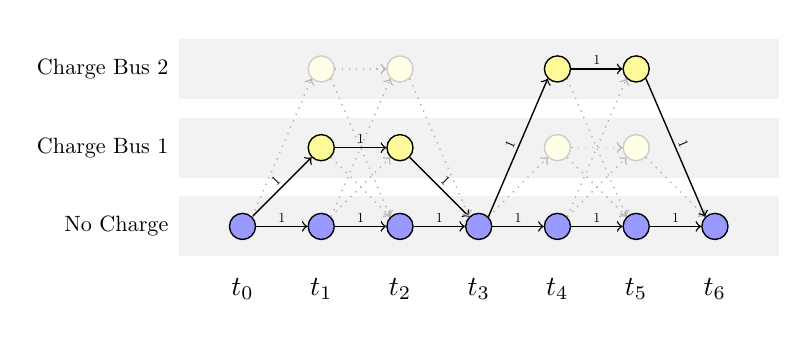
\begin{tikzpicture} 
		\node[rectangle, fill=gray!10, minimum width=3in, minimum height=.3in,label=left:\scalebox{0.8}{Charge Bus 2}](bus2Box) at (3,1){};
		\node[rectangle, fill=gray!10, minimum width=3in, minimum height=.3in,label=left:\scalebox{0.8}{Charge Bus 1}](bus1Box) at (3,0){};
		\node[rectangle, fill=gray!10, minimum width=3in, minimum height=.3in,label=left:\scalebox{0.8}{No Charge}](bus1Box) at (3,-1){};

		\node[circle, fill=yellow!40, line width=0.5pt, draw=black, minimum size=0.1in](two) at (1,0){}; 
		\node[circle, fill=yellow!40, line width=0.5pt, draw=black, minimum size=0.1in](three) at (2,0){};
		\node[circle, fill=yellow!10, line width=0.5pt, draw=black!20, minimum size=0.1in](five) at (4,0){};
		\node[circle, fill=yellow!10, line width=0.5pt, draw=black!20, minimum size=0.1in](six) at (5,0){};

		\node[circle, fill=yellow!10, line width=0.5pt, draw=black!20, minimum size=0.1in](nine) at (1,1){}; 
		\node[circle, fill=yellow!10, line width=0.5pt, draw=black!20, minimum size=0.1in](ten) at (2,1){};
		\node[circle, fill=yellow!40, line width=0.5pt, draw=black, minimum size=0.1in](twelve) at (4,1){};
		\node[circle, fill=yellow!40, line width=0.5pt, draw=black, minimum size=0.1in](thirteen) at (5,1){};

		\node[circle, fill=blue!40, line width=0.5pt, draw=black, minimum size=0.1in](bOne) at (0,-1){};
		\node[circle, fill=blue!40, line width=0.5pt, draw=black, minimum size=0.1in](bTwo) at (1,-1){}; 
		\node[circle, fill=blue!40, line width=0.5pt, draw=black, minimum size=0.1in](bThree) at (2,-1){};
		\node[circle, fill=blue!40, line width=0.5pt, draw=black, minimum size=0.1in](bFour) at (3,-1){};
		\node[circle, fill=blue!40, line width=0.5pt, draw=black, minimum size=0.1in](bFive) at (4,-1){};
		\node[circle, fill=blue!40, line width=0.5pt, draw=black, minimum size=0.1in](bSix) at (5,-1){};
		\node[circle, fill=blue!40, line width=0.5pt, draw=black, minimum size=0.1in](bSeven) at (6,-1){};

		\node[rectangle, minimum width=0.3in, minimum height=1.2in,label=below:$t_0$](time0Box) at (0,0){};
		\node[rectangle, minimum width=0.3in, minimum height=1.2in,label=below:$t_1$](time1Box) at (1,0){};
		\node[rectangle, minimum width=0.3in, minimum height=1.2in,label=below:$t_2$](time2Box) at (2,0){};
		\node[rectangle, minimum width=0.3in, minimum height=1.2in,label=below:$t_3$](time3Box) at (3,0){};
		\node[rectangle, minimum width=0.3in, minimum height=1.2in,label=below:$t_4$](time4Box) at (4,0){};
		\node[rectangle, minimum width=0.3in, minimum height=1.2in,label=below:$t_5$](time5Box) at (5,0){};
		\node[rectangle, minimum width=0.3in, minimum height=1.2in,label=below:$t_6$](time6Box) at (6,0){}; 
		
		% draw rest edges
		\draw[->, line width=0.5pt] (bOne.east) -- node [text width=2.5cm, midway, above=-2.1pt, align=center]{\scalebox{0.5}{1}}(bTwo.west);
		\draw[->, line width=0.5pt] (bTwo.east) -- node [text width=2.5cm, midway, above=-2.1pt, align=center]{\scalebox{0.5}{1}}(bThree.west);
		\draw[->, line width=0.5pt] (bThree.east) -- node [text width=2.5cm, midway, above=-2.1pt, align=center]{\scalebox{0.5}{1}}(bFour.west);
		\draw[->, line width=0.5pt] (bFour.east) -- node [text width=2.5cm, midway, above=-2.1pt, align=center]{\scalebox{0.5}{1}}(bFive.west);
		\draw[->, line width=0.5pt] (bFive.east) -- node [text width=2.5cm, midway, above=-2.1pt, align=center]{\scalebox{0.5}{1}}(bSix.west);
		\draw[->, line width=0.5pt] (bSix.east) -- node [text width=2.5cm, midway, above=-2.1pt, align=center]{\scalebox{0.5}{1}}(bSeven.west);
		
		% draw connect edges
		\draw[->, line width=0.5pt] (bOne.north east) -- node [sloped, text width=2.5cm, midway, above=-2.1pt, align=center]{\scalebox{0.5}{1}}(two.south west); 
		\draw[->, dotted, color=black!30, line width=0.5pt] (bTwo.north east) -- (three.south west);
		\draw[->, dotted, color=black!30, line width=0.5pt] (bFour.north east) -- (five.south west);
		\draw[->, dotted, color=black!30, line width=0.5pt] (bFive.north east) -- (six.south west);

		\draw[->, dotted, color=black!30, line width=0.5pt] (bOne.north east) -- (nine.south west);
		\draw[->, dotted, color=black!30, line width=0.5pt] (bTwo.north east) -- (ten.south west);
		\draw[->, line width=0.5pt] (bFour.north east) -- node [sloped, text width=2.5cm, midway, above=-2.1pt, align=center]{\scalebox{0.5}{1}}(twelve.south west);
		\draw[->, dotted, color=black!30, line width=0.5pt] (bFive.north east) -- (thirteen.south west);

		% draw disconnect edges
		\draw[->, dotted, color=black!30, line width=0.5pt] (two.south east) -- (bThree.north west); 
		\draw[->, line width=0.5pt] (three.south east) -- node [sloped, text width=2.5cm, midway, above=-2.1pt, align=center]{\scalebox{0.5}{1}}(bFour.north west);
		\draw[->, dotted, color=black!30, line width=0.5pt] (five.south east) -- (bSix.north west);
		\draw[->, dotted, color=black!30, line width=0.5pt] (six.south east) -- (bSeven.north west);

		\draw[->, dotted, color=black!30, line width=0.5pt] (nine.south east) -- (bThree.north west);
		\draw[->, dotted, color=black!30, line width=0.5pt] (ten.south east) -- (bFour.north west);
		\draw[->, dotted, color=black!30, line width=0.5pt] (twelve.south east) -- (bSix.north west);
		\draw[->, line width=0.5pt] (thirteen.south east) -- node [sloped, text width=2.5cm, midway, above=-2.1pt, align=center]{\scalebox{0.5}{1}}(bSeven.north west);

		% draw charge edges
		\draw[->, line width=0.5pt] (two.east) -- node [text width=2.5cm, midway, above=-2.1pt, align=center]{\scalebox{0.5}{1}}(three.west);
		\draw[->, dotted, color=black!30, line width=0.5pt] (five.east) -- (six.west);
		\draw[->, dotted, color=black!30, line width=0.5pt] (nine.east) -- (ten.west);
		\draw[->, line width=0.5pt] (twelve.east) -- node [text width=2.5cm, midway, above=-2.1pt, align=center]{\scalebox{0.5}{1}}(thirteen.west); 
	\end{tikzpicture}
	\caption{One solution to a 2-bus 2-charger scenario}
	\label{fig:graphWithSolution}
\end{figure}



\par To find the optimal set of weights, the graph must first be encoded in an incidence matrix. An incidence matrix organizes relationships between nodes and edges by describing which edges depart from and connect to which nodes. An incidence matrix $A$ is an nNode $\times$ nEdge matrix where nNode is the number of nodes, and nEdge is the number of edges. 
\par The columns of $A$ describe connections for each edge and the rows give connections for each node. Incoming connections are represented with $1$, outgoing connections with $-1$, and no connection with $0$. For example, the graph in figure \ref{fig:genericGraph} can be represented as:
\begin{figure}
	\centering
	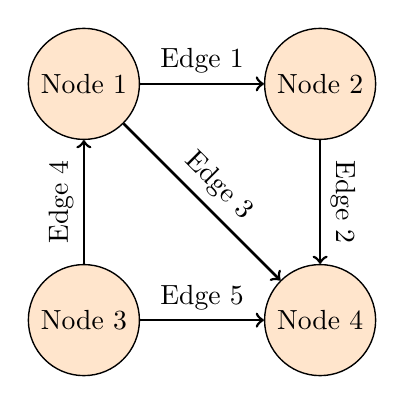
\begin{tikzpicture}
		\node[circle, line width=0.5pt, draw=black, fill=orange!20, minimum size=0.5in](topLeft) at (0,3){Node 1};
		\node[circle, line width=0.5pt, draw=black, fill=orange!20, minimum size=0.5in](topRight) at (3,3){Node 2};
		\node[circle, line width=0.5pt, draw=black, fill=orange!20, minimum size=0.5in](btmLeft) at (0,0){Node 3};
		\node[circle, line width=0.5pt, draw=black, fill=orange!20, minimum size=0.5in](btmRight) at (3,0){Node 4};
		\draw [->, line width=1pt] (topLeft.east) -- node [text width=2.5cm, midway, above, align=center]{Edge 1}(topRight.west);
		\draw [->, line width=1pt] (btmLeft.north) -- node [sloped, anchor=center, above, text width=2.5cm, midway, align=center]{Edge 4}(topLeft.south);
		\draw [->, line width=1pt] (topLeft.south east) -- node [sloped, anchor=center, above, text width=2.5cm, midway, align=center]{Edge 3}(btmRight.north west);
		\draw [->, line width=1pt] (topRight.south) -- node[sloped, anchor=center, above, text width=2.5cm, midway, align=center]{Edge 2}(btmRight.north);
		\draw [->, line width=1pt] (btmLeft.east) -- node[text width=2.5cm, midway, above, align=center]{Edge 5}(btmRight.west);
	\end{tikzpicture}
	\caption{A generic directed graph consisting of nodes and edges}
	\label{fig:genericGraph}
\end{figure}
\begin{align}
	\begin{bmatrix}
		-1 & 0 & -1 & 1 & 0 \\
		1 & -1 & 0 & 0 & 0 \\
		0 & 0 & 0 & -1 & -1 \\
		0 & 1 & 1 & 0 & 1 \\
	\end{bmatrix}
\end{align}
\par  An incidence matrix can be used to find the number of chargers entering and leaving each state. None of the states (charging/non-charging) can create or destroy chargers and so the number of incoming must always equal the number of outgoing chargers. The only exception occurs at \textit{source} and \textit{sink} nodes.
\par A source node represents the beginning state of all chargers.  Because a source state is the first, there are no incoming edges and hence, the net difference between incoming and outgoing chargers, or \textit{the net-flow}, will be minus the number of chargers. 
\par Sink nodes represent the final state, where all chargers enter and finish (see figure \ref{fig:sourceSink}). Because sinks have no outgoing edges, they maintain a positive net-flow equal to the number of chargers. Let $x$ be a vector representing the edge weights, $A$ be an adjacency matrix, and $f$ be a vector where $f_i$ gives the net-flow for the $i^{\text{th}}$ node. The net-flow for each node can be expressed as 

\begin{figure}
	\centering
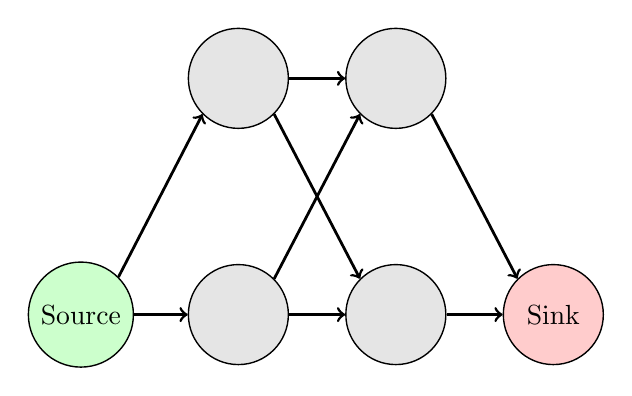
\begin{tikzpicture}
	\node[circle, fill=green!20, line width=0.5pt, draw=black, minimum size=0.5in](one) at (0,0){Source};
	\node[circle, fill=gray!20,line width=0.5pt, draw=black, minimum size=0.5in](two) at (2,0){};
	\node[circle, fill=gray!20,line width=0.5pt, draw=black, minimum size=0.5in](three) at (4,0){};
	\node[circle, fill=red!20,line width=0.5pt, draw=black, minimum size=0.5in](four) at (6,0){Sink};
	\node[circle, fill=gray!20, line width=0.5pt, draw=black, minimum size=0.5in](five) at (2,3){};
	\node[circle, fill=gray!20, line width=0.5pt, draw=black, minimum size=0.5in](six) at (4,3){};
	\draw [->, line width=1pt] (one.north east) -- (five.south west);
	\draw [->, line width=1pt] (one.east) -- (two.west);
	\draw [->, line width=1pt] (five.east) -- (six.west);
	\draw [->, line width=1pt] (five.south east) -- (three.north west);
	\draw [->, line width=1pt] (two.north east) -- (six.south west);
	\draw [->, line width=1pt] (six.south east) -- (four.north west);
	\draw [->, line width=1pt] (two.east) -- (three.west);
	\draw [->, line width=1pt] (three.east) -- (four.west); 
\end{tikzpicture}
	\caption{Network flow illustrating sources and sinks}
	\label{fig:sourceSink} 
\end{figure} 

\begin{align}
	Ax = f
\end{align}
This expression can be used to constrain the net-flow of each node.  $f$ must equal zero for all non-source and non-sink elements and source/sink nodes must have net-flows equal to $-\text{nChargers}$ and nChargers respectively (see equation \ref{eqn:cFlow}).
\begin{align}\label{eqn:cFlow}
	Ax = \begin{bmatrix} 0 \\ \vdots \\ -\text{nCharger} \\ \vdots \\ 0 \\ \text{nCharger} \\ \vdots \\ 0\end{bmatrix}
\end{align}

\par Flow can also be used to ensure that buses connect to only one charger at a time. Let a charge session, or \textit{group}, be the set of all charge nodes between routes as shown in figure \ref{fig:groups}. The \textit{group flow} is the number of chargers that enter a group and is computed by adding the weights for all incoming edges (see figure \ref{fig:groupedEdges}). 
\par Let $B$ be a nGroup $\times$ nEdge matrix where the $ij^{\text{th}}$ entry is $1$ if the $j^{\text{th}}$ edge enters the $i^{\text{th}}$ group and $0$ otherwise. For example, the $B$ matrix corresponding to figure \ref{fig:groupEdges} contains $1$ in the $7^{\text{th}}$ and $10^{\text{th}}$ columns for Group 1, and $12^{\text{th}}$ and $15^{\text{th}}$ columns for group 2 as given in equation \ref{eqn:groupB}.
\begin{align}\label{eqn:groupB}
	B = \begin{bmatrix}0 & 0 & 0 & 0 & 0 & 0 & 1 & 0 & 0 & 1 & 0 & 0 & 0 & 0 & 0 & 0\\
	                   0 & 0 & 0 & 0 & 0 & 0 & 0 & 0 & 0 & 0 & 0 & 1 & 0 & 0 & 1 & 0\end{bmatrix}
\end{align}

\begin{figure}
	\centering
	\begin{tikzpicture}
		\node[circle, fill=blue!20, line width=0.5pt, draw=black, minimum size=0.1in](one) at (0,0){};
		\node[circle, fill=blue!20, line width=0.5pt, draw=black, minimum size=0.1in](two) at (1,0){}; 
		\node[circle, fill=blue!20, line width=0.5pt, draw=black, minimum size=0.1in](three) at (2,0){};
		\node[circle, fill=blue!20, line width=0.5pt, draw=black, minimum size=0.1in](four) at (3,0){};
		\node[circle, fill=blue!20, line width=0.5pt, draw=black, minimum size=0.1in](five) at (4,0){};
		\node[circle, fill=blue!20, line width=0.5pt, draw=black, minimum size=0.1in](six) at (5,0){};
		\node[circle, fill=blue!20, line width=0.5pt, draw=black, minimum size=0.1in](seven) at (6,0){};
		\node[circle, fill=yellow!20, line width=0.5pt, draw=black, minimum size=0.1in](eight) at (1,2){};
		\node[circle, fill=yellow!20, line width=0.5pt, draw=black, minimum size=0.1in](nine) at (2,2){};
		\node[circle, fill=yellow!20, line width=0.5pt, draw=black, minimum size=0.1in](ten) at (4,2){}; 
		\node[circle, fill=yellow!20, line width=0.5pt, draw=black, minimum size=0.1in](eleven) at (5,2){}; 
		\node[ellipse, line width=0.5pt, draw=red, minimum height=0.4in, minimum width=1in, label=Group 1](group1) at (1.5,2){};
		\node[ellipse, line width=0.5pt, draw=red, minimum height=0.4in, minimum width=1in, label=Group 2](group2) at (4.5,2){};
		\draw [->, line width=0.5pt] (one.east) -- (two.west);
		\draw [->, line width=0.5pt] (two.east) -- (three.west);
		\draw [->, line width=0.5pt] (three.east) -- (four.west);
		\draw [->, line width=0.5pt] (four.east) -- (five.west);
		\draw [->, line width=0.5pt] (five.east) -- (six.west);
		\draw [->, line width=0.5pt] (six.east) -- (seven.west);
		\draw [->, line width=0.5pt] (one.north east) -- (eight.south west);
		\draw [->, line width=0.5pt] (two.north east) -- (nine.south west);
		\draw [->, line width=0.5pt] (four.north east) -- (ten.south west);
		\draw [->, line width=0.5pt] (five.north east) -- (eleven.south west);
		\draw [->, line width=0.5pt] (eight.south east) -- (three.north west);
		\draw [->, line width=0.5pt] (nine.south east) -- (four.north west);
		\draw [->, line width=0.5pt] (ten.south east) -- (six.north west);
		\draw [->, line width=0.5pt] (eleven.south east) -- (seven.north west);
		\draw [->, line width=0.5pt] (eight.east) -- (nine.west);
		\draw [->, line width=0.5pt] (ten.east) -- (eleven.west); 
	\end{tikzpicture}
	\caption{Example of groups in a network flow graph}
	\label{fig:groups}
\end{figure}
\begin{figure}
\centering
	\begin{tikzpicture}
		\node[circle, fill=blue!20, line width=0.5pt, draw=black, minimum size=0.1in](one) at (0,0){};
		\node[circle, fill=blue!20, line width=0.5pt, draw=black, minimum size=0.1in](two) at (1,0){}; 
		\node[circle, fill=blue!20, line width=0.5pt, draw=black, minimum size=0.1in](three) at (2,0){};
		\node[circle, fill=blue!20, line width=0.5pt, draw=black, minimum size=0.1in](four) at (3,0){};
		\node[circle, fill=blue!20, line width=0.5pt, draw=black, minimum size=0.1in](five) at (4,0){};
		\node[circle, fill=blue!20, line width=0.5pt, draw=black, minimum size=0.1in](six) at (5,0){};
		\node[circle, fill=blue!20, line width=0.5pt, draw=black, minimum size=0.1in](seven) at (6,0){};
		\node[circle, fill=yellow!20, line width=0.5pt, draw=black, minimum size=0.1in](eight) at (1,2){};
		\node[circle, fill=yellow!20, line width=0.5pt, draw=black, minimum size=0.1in](nine) at (2,2){};
		\node[circle, fill=yellow!20, line width=0.5pt, draw=black, minimum size=0.1in](ten) at (4,2){}; 
		\node[circle, fill=yellow!20, line width=0.5pt, draw=black, minimum size=0.1in](eleven) at (5,2){}; 
		\draw [->, line width=0.5pt,color=black!40] (one.east) -- (two.west);
		\draw [->, line width=0.5pt,color=black!40] (two.east) -- (three.west);
		\draw [->, line width=0.5pt,color=black!40] (three.east) -- (four.west);
		\draw [->, line width=0.5pt,color=black!40] (four.east) -- (five.west);
		\draw [->, line width=0.5pt,color=black!40] (five.east) -- (six.west);
		\draw [->, line width=0.5pt,color=black!40] (six.east) -- (seven.west);
		\draw [->, color=orange, line width=0.75pt] (one.north east) -- (eight.south west);
		\draw [->, color=orange, line width=0.75pt] (two.north east) -- (nine.south west);
		\draw [->, color=purple, line width=0.75pt] (four.north east) -- (ten.south west);
		\draw [->, color=purple, line width=0.75pt] (five.north east) -- (eleven.south west);
		\draw [->, line width=0.5pt,color=black!40] (eight.south east) -- (three.north west);
		\draw [->, line width=0.5pt,color=black!40] (nine.south east) -- (four.north west);
		\draw [->, line width=0.5pt,color=black!40] (ten.south east) -- (six.north west);
		\draw [->, line width=0.5pt,color=black!40] (eleven.south east) -- (seven.north west);
		\draw [->, line width=0.5pt,color=black!40] (eight.east) -- (nine.west);
		\draw [->, line width=0.5pt,color=black!40] (ten.east) -- (eleven.west); 
		\node[ellipse, line width=0pt, draw opacity=0.5, fill opacity=0.2, fill=purple!40, draw=purple!40, minimum height=0.4in, minimum width=1in, label=Group 2](group2) at (4.5,2){};
		\node[ellipse, line width=0pt, draw opacity=0.5, fill opacity=0.2, fill=orange!40, draw=orange!40, minimum height=0.4in, minimum width=1in, label=Group 1](group1) at (1.5,2){};
	\end{tikzpicture}
	\caption{Incoming Group Edges}
	\label{fig:groupedEdges} 
\end{figure} 
The group flow is then computed as 
\begin{align}
	Bx = \text{Group Flow}.
\end{align}
But the group flow is required to be one at most.  This is expressed by the inequality given in equation \ref{eqn:cGroupFlow}.
\begin{align}\label{eqn:cGroupFlow}
	Bx \le \begin{bmatrix} 1\\ 1 \\\vdots \\ 1\end{bmatrix},
\end{align}
where $x$ is a matrix giving the number of chargers traversing an edge, and $B$ describes all mount edges (see figure \ref{fig:edgeTypes}) corresponding to the same group. In $B$, the i,jth value is one if the jth edge mounts to the ith group.  For example, the graph given in figure \ref{fig:groupEdges} would have the following group constraints:


\begin{figure}
\centering
	\begin{tikzpicture}
		\node[circle, fill=blue!20, line width=0.5pt, draw=black, minimum size=0.1in](one) at (0,0){};
		\node[circle, fill=blue!20, line width=0.5pt, draw=black, minimum size=0.1in](two) at (1,0){}; 
		\node[circle, fill=blue!20, line width=0.5pt, draw=black, minimum size=0.1in](three) at (2,0){};
		\node[circle, fill=blue!20, line width=0.5pt, draw=black, minimum size=0.1in](four) at (3,0){};
		\node[circle, fill=blue!20, line width=0.5pt, draw=black, minimum size=0.1in](five) at (4,0){};
		\node[circle, fill=blue!20, line width=0.5pt, draw=black, minimum size=0.1in](six) at (5,0){};
		\node[circle, fill=blue!20, line width=0.5pt, draw=black, minimum size=0.1in](seven) at (6,0){};
		\node[circle, fill=yellow!20, line width=0.5pt, draw=black, minimum size=0.1in](eight) at (1,2){};
		\node[circle, fill=yellow!20, line width=0.5pt, draw=black, minimum size=0.1in](nine) at (2,2){};
		\node[circle, fill=yellow!20, line width=0.5pt, draw=black, minimum size=0.1in](ten) at (4,2){}; 
		\node[circle, fill=yellow!20, line width=0.5pt, draw=black, minimum size=0.1in](eleven) at (5,2){}; 
		\node[ellipse, line width=0pt, draw=white, minimum height=0.4in, minimum width=1in, label=Group 1](group1) at (1.5,2){};
		\node[ellipse, line width=0pt, draw=white, minimum height=0.4in, minimum width=1in, label=Group 2](group2) at (4.5,2){};
		\draw [->, line width=0.5pt,color=black!40] (one.east) -- (two.west);
		\draw [->, line width=0.5pt,color=black!40] (two.east) -- (three.west);
		\draw [->, line width=0.5pt,color=black!40] (three.east) -- (four.west);
		\draw [->, line width=0.5pt,color=black!40] (four.east) -- (five.west);
		\draw [->, line width=0.5pt,color=black!40] (five.east) -- (six.west);
		\draw [->, line width=0.5pt,color=black!40] (six.east) -- (seven.west);
		\draw [->, color=orange, line width=0.75pt] (one.north east) -- node[sloped, anchor=center, above, text width=2.5cm, align=center]{Edge 7}(eight.south west);
		\draw [->, color=orange, line width=0.75pt] (two.north east) -- node[sloped, anchor=center, above, text width=2.5cm, align=center]{Edge 10}(nine.south west);
		\draw [->, color=purple, line width=0.75pt] (four.north east) -- node[sloped, anchor=center, above, text width=2.5cm, align=center]{Edge 12}(ten.south west);
		\draw [->, color=purple, line width=0.75pt] (five.north east) -- node[sloped, anchor=center, above, text width=2.5cm, align=center]{Edge 15}(eleven.south west);
		\draw [->, line width=0.5pt,color=black!40] (eight.south east) -- (three.north west);
		\draw [->, line width=0.5pt,color=black!40] (nine.south east) -- (four.north west);
		\draw [->, line width=0.5pt,color=black!40] (ten.south east) -- (six.north west);
		\draw [->, line width=0.5pt,color=black!40] (eleven.south east) -- (seven.north west);
		\draw [->, line width=0.5pt,color=black!40] (eight.east) -- (nine.west);
		\draw [->, line width=0.5pt,color=black!40] (ten.east) -- (eleven.west); 
	\end{tikzpicture}
	\caption{Connect edge example for groups}
	\label{fig:groupEdges} 
\end{figure} 
\section{Multi-Graph Additions}
An additional contribution this work offers is the expansion to night vs day charging. During the night, there is one charger for each bus; each with a single charge rate.  During this time, buses are also available to charge at any time.  These differences in operations introduce changes to the original graph formation and warrent a separate graph.  
\par Night graphs consider a situation where both the number of buses reflecte the number of chargers and buses are readily available.  Note how there are several source and sink nodes in figure \ref{fig:nightVsDayGraph}.  When a bus deploys for the day, the available number of charges changes and are reflected in the underlying source and sink constraints.
\begin{figure*}
	\centering
	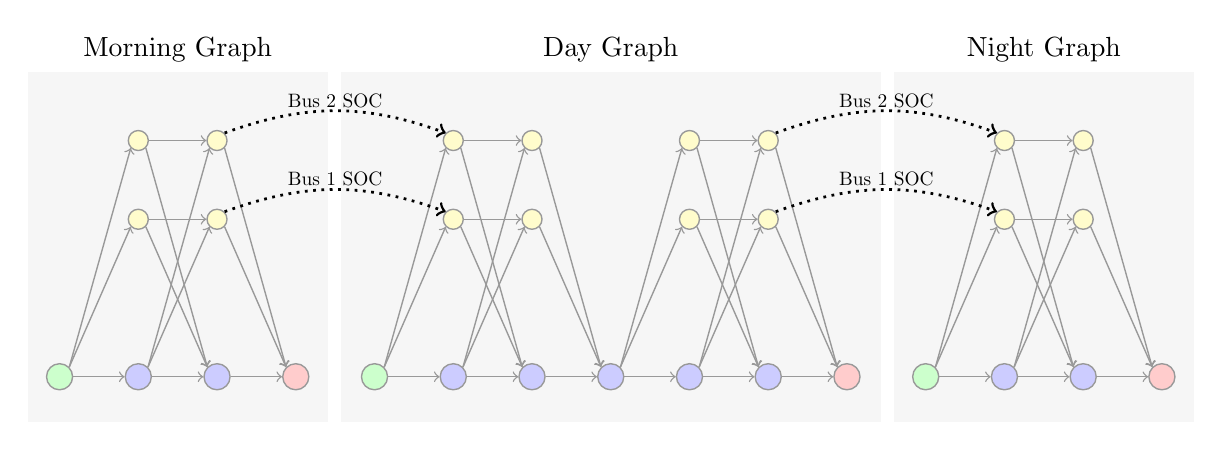
\begin{tikzpicture} 
		% morning graph
		\node[rectangle, fill=gray!7, minimum width=1.5in, minimum height=1.75in, label=above:Morning Graph](mBox) at (-2.5,1.65){};
		\node[circle, fill=green!20, line width=0.5pt, draw=black!40, minimum size=0.1in](mOne) at (-4,0){};
		\node[circle, fill=blue!20, line width=0.5pt, draw=black!40, minimum size=0.1in](mTwo) at (-3,0){}; 
		\node[circle, fill=blue!20, line width=0.5pt, draw=black!40, minimum size=0.1in](mThree) at (-2,0){};
		\node[circle, fill=red!20, line width=0.5pt, draw=black!40, minimum size=0.1in](mFour) at (-1,0){};

		\node[circle, fill=yellow!20, line width=0.5pt, draw=black!40, minimum size=0.1in, inner sep=1pt](mFive) at (-3,2){};
		\node[circle, fill=yellow!20, line width=0.5pt, draw=black!40, minimum size=0.1in, inner sep=1pt](mSix) at (-2,2){};
		\node[circle, fill=yellow!20, line width=0.5pt, draw=black!40, minimum size=0.1in, inner sep=1pt](mSeven) at (-3,3){};
		\node[circle, fill=yellow!20, line width=0.5pt, draw=black!40, minimum size=0.1in, inner sep=1pt](mEight) at (-2,3){};

		\draw[->, line width=0.5pt, color=black!40] (mOne.east) -- (mTwo.west){};
		\draw[->, line width=0.5pt, color=black!40] (mTwo.east) -- (mThree.west){};
		\draw[->, line width=0.5pt, color=black!40] (mThree.east) -- (mFour.west){};

		\draw[->, line width=0.5pt, color=black!40] (mOne.north east) -- (mFive.south west){};
		\draw[->, line width=0.5pt, color=black!40] (mTwo.north east) -- (mSix.south west){};
		\draw[->, line width=0.5pt, color=black!40] (mOne.north east) -- (mSeven.south west){};
                \draw[->, line width=0.5pt, color=black!40] (mTwo.north east) -- (mEight.south west){};

                \draw[->, line width=0.5pt, color=black!40] (mFive.south east) -- (mThree.north west){}; 
                \draw[->, line width=0.5pt, color=black!40] (mSix.south east) -- (mFour.north west){};
                \draw[->, line width=0.5pt, color=black!40] (mSeven.south east) -- (mThree.north west){};
		\draw[->, line width=0.5pt, color=black!40] (mEight.south east) -- (mFour.north west){};

                \draw[->, line width=0.5pt, color=black!40] (mFive.east) -- (mSix.west){};
                \draw[->, line width=0.5pt, color=black!40] (mSeven.east) -- (mEight.west){};

		% night graph
		\node[rectangle, fill=gray!7, minimum width=1.5in, minimum height=1.75in, label=above:Night Graph](nBox) at (8.5,1.65){};
		\node[circle, fill=green!20, line width=0.5pt, draw=black!40, minimum size=0.1in](nOne) at (7,0){};
		\node[circle, fill=blue!20, line width=0.5pt, draw=black!40, minimum size=0.1in](nTwo) at (8,0){}; 
		\node[circle, fill=blue!20, line width=0.5pt, draw=black!40, minimum size=0.1in](nThree) at (9,0){};
		\node[circle, fill=red!20, line width=0.5pt, draw=black!40, minimum size=0.1in](nFour) at (10,0){};

		\node[circle, fill=yellow!20, line width=0.5pt, draw=black!40, minimum size=0.1in, inner sep=1pt](nFive) at (8,2){};
		\node[circle, fill=yellow!20, line width=0.5pt, draw=black!40, minimum size=0.1in, inner sep=1pt](nSix) at (9,2){};
		\node[circle, fill=yellow!20, line width=0.5pt, draw=black!40, minimum size=0.1in, inner sep=1pt](nSeven) at (8,3){};
		\node[circle, fill=yellow!20, line width=0.5pt, draw=black!40, minimum size=0.1in, inner sep=1pt](nEight) at (9,3){};

		\draw[->, line width=0.5pt, color=black!40] (nOne.east) -- (nTwo.west){};
		\draw[->, line width=0.5pt, color=black!40] (nTwo.east) -- (nThree.west){};
		\draw[->, line width=0.5pt, color=black!40] (nThree.east) -- (nFour.west){};

		\draw[->, line width=0.5pt, color=black!40] (nOne.north east) -- (nFive.south west){};
		\draw[->, line width=0.5pt, color=black!40] (nTwo.north east) -- (nSix.south west){};
		\draw[->, line width=0.5pt, color=black!40] (nOne.north east) -- (nSeven.south west){};
                \draw[->, line width=0.5pt, color=black!40] (nTwo.north east) -- (nEight.south west){};

                \draw[->, line width=0.5pt, color=black!40] (nFive.south east) -- (nThree.north west){}; 
                \draw[->, line width=0.5pt, color=black!40] (nSix.south east) -- (nFour.north west){};
		\draw[->, line width=0.5pt, color=black!40] (nSeven.south east) -- (nThree.north west){};
		\draw[->, line width=0.5pt, color=black!40] (nEight.south east) -- (nFour.north west){};

		\draw[->, line width=0.5pt, color=black!40] (nFive.east) -- (nSix.west){};
                \draw[->, line width=0.5pt, color=black!40] (nSeven.east) -- (nEight.west){};


		% day graph	
		\node[rectangle, fill=gray!7, minimum width=2.7in, minimum height=1.75in, label=above:Day Graph](dBox) at (3,1.65){}; 
		\node[circle, fill=green!20, line width=0.5pt, draw=black!40, minimum size=0.1in](one) at (0,0){};
		\node[circle, fill=blue!20, line width=0.5pt, draw=black!40, minimum size=0.1in](two) at (1,0){}; 
		\node[circle, fill=blue!20, line width=0.5pt, draw=black!40, minimum size=0.1in](three) at (2,0){};
		\node[circle, fill=blue!20, line width=0.5pt, draw=black!40, minimum size=0.1in](four) at (3,0){};
		\node[circle, fill=blue!20, line width=0.5pt, draw=black!40, minimum size=0.1in](five) at (4,0){};
		\node[circle, fill=blue!20, line width=0.5pt, draw=black!40, minimum size=0.1in](six) at (5,0){};
		\node[circle, fill=red!20, line width=0.5pt, draw=black!40, minimum size=0.1in](seven) at (6,0){};
		
		\node[circle, fill=yellow!20, line width=0.5pt, draw=black!40, minimum size=0.1in, inner sep=1pt](eight) at (1,2){};
		\node[circle, fill=yellow!20, line width=0.5pt, draw=black!40, minimum size=0.1in, inner sep=1pt](nine) at (2,2){};
		\node[circle, fill=yellow!20, line width=0.5pt, draw=black!40, minimum size=0.1in, inner sep=1pt](ten) at (4,2){};
		\node[circle, fill=yellow!20, line width=0.5pt, draw=black!40, minimum size=0.1in, inner sep=1pt](eleven) at (5,2){};

		\node[circle, fill=yellow!20, line width=0.5pt, draw=black!40, minimum size=0.1in, inner sep=1pt](twelve) at (1,3){};
		\node[circle, fill=yellow!20, line width=0.5pt, draw=black!40, minimum size=0.1in, inner sep=1pt](thirteen) at (2,3){};
		\node[circle, fill=yellow!20, line width=0.5pt, draw=black!40, minimum size=0.1in, inner sep=1pt](fourteen) at (4,3){};
		\node[circle, fill=yellow!20, line width=0.5pt, draw=black!40, minimum size=0.1in, inner sep=1pt](fifteen) at (5,3){};

		\draw [->, line width=0.5pt, color=black!40] (one.east) -- (two.west);
		\draw [->, line width=0.5pt, color=black!40] (two.east) -- (three.west);
		\draw [->, line width=0.5pt, color=black!40] (three.east) -- (four.west);
		\draw [->, line width=0.5pt, color=black!40] (four.east) -- (five.west);
		\draw [->, line width=0.5pt, color=black!40] (five.east) -- (six.west);
		\draw [->, line width=0.5pt, color=black!40] (six.east) -- (seven.west);

		\draw [->, line width=0.5pt, color=black!40] (one.north east) -- (eight.south west);
		\draw [->, line width=0.5pt, color=black!40] (two.north east) -- (nine.south west);
		\draw [->, line width=0.5pt, color=black!40] (four.north east) -- (ten.south west);
		\draw [->, line width=0.5pt, color=black!40] (five.north east) -- (eleven.south west);
		\draw [->, line width=0.5pt, color=black!40] (eight.south east) -- (three.north west);
		\draw [->, line width=0.5pt, color=black!40] (nine.south east) -- (four.north west);
		\draw [->, line width=0.5pt, color=black!40] (ten.south east) -- (six.north west);
		\draw [->, line width=0.5pt, color=black!40] (eleven.south east) -- (seven.north west);
		\draw [->, line width=0.5pt, color=black!40] (eight.east) -- (nine.west);
		\draw [->, line width=0.5pt, color=black!40] (ten.east) -- (eleven.west); 

		\draw [->, line width=0.5pt, color=black!40] (one.north east) -- (twelve.south west);
		\draw [->, line width=0.5pt, color=black!40] (two.north east) -- (thirteen.south west);
		\draw [->, line width=0.5pt, color=black!40] (four.north east) -- (fourteen.south west);
		\draw [->, line width=0.5pt, color=black!40] (five.north east) -- (fifteen.south west);
		\draw [->, line width=0.5pt, color=black!40] (twelve.south east) -- (three.north west);
		\draw [->, line width=0.5pt, color=black!40] (thirteen.south east) -- (four.north west);
		\draw [->, line width=0.5pt, color=black!40] (fourteen.south east) -- (six.north west);
		\draw [->, line width=0.5pt, color=black!40] (fifteen.south east) -- (seven.north west);
		\draw [->, line width=0.5pt, color=black!40] (twelve.east) -- (thirteen.west);
		\draw [->, line width=0.5pt, color=black!40] (fourteen.east) -- (fifteen.west); 


		\draw [dotted, color=black,-,line width=1pt] (mSix.north east) edge[->,bend left=20pt]node[above=-2.5pt]{\scalebox{0.7}{Bus 1 SOC}}(eight.north west); 
		\draw [dotted, color=black,-,line width=1pt] (mEight.north east) edge[->,bend left=20pt]node[above=-2.5pt]{\scalebox{0.7}{Bus 2 SOC}}(twelve.north west);

		\draw [dotted, color=black,-,line width=1pt] (eleven.north east) edge[->,bend left=20pt]node[above=-2.5pt]{\scalebox{0.7}{Bus 1 SOC}}(nFive.north west); 
		\draw [dotted, color=black,-,line width=1pt] (fifteen.north east) edge[->,bend left=20pt]node[above=-2.5pt]{\scalebox{0.7}{Bus 2 SOC}}(nSeven.north west);
	\end{tikzpicture}
	\caption{Night vs Day Graphs}
	\label{fig:nightVsDayGraph}
\end{figure*}
\par Changes in the first graph are reflected in the second through use of state of charge variables.
